\documentclass{report}
\usepackage{a4}
\usepackage[latin1]{inputenc}
%\usepackage[dvips]{graphicx}
\usepackage[pdftex]{graphicx}
\usepackage{verbatim}
\usepackage[total={6in, 9in}, top=1in,left=1.1in]{geometry} 
\usepackage{moreverb}
\usepackage{psfrag}
\usepackage{amsmath}
\usepackage[small]{caption}
\usepackage{amssymb}
\usepackage{fancyhdr}
\usepackage{shadow}            
\usepackage{setspace}
\usepackage{listings}
\usepackage{subfig}
\usepackage{upquote} %To make straigh quotes work in pdf
\usepackage[dvipsnames]{xcolor}
\definecolor{mygreen}{RGB}{0,102,51}
\definecolor{mycer}{RGB}{42, 82, 190 }
\definecolor{myred}{RGB}{102, 0, 0 }
\definecolor{mygray}{gray}{0.85}

\setlength{\headheight}{12.5pt}
\newcommand{\undertilde}[1]{\underset{\widetilde{}}{#1}}
\newcommand{\HRule}{\rule{\linewidth}{0.5mm}}

\pagestyle{fancy}


\begin{document}

 \begin{titlepage}
  \begin{center}
 
 
	

	

        \HRule \\[0.4cm]
        Tutorial:\\[0.2cm]
	{ \huge \bfseries GMSH Introduction Tutorial}\\[0.4cm]
	\HRule \\[1cm]

        \begin{minipage}{0.35\textwidth}
        Developed using gmsh 4.7+ \newline \newline \newline \newline \newline \newline \newline \\
	\end{minipage}\\[1cm]

	

	\includegraphics[width=15cm]{TSDA_title.png}
	
	\vfill


	{\large \today}
	 
	\end{center}

 \end{titlepage}


\chapter*{Learning outcomes}

\noindent The reader will learn:\\[0.4cm]

\noindent{\bf How to use it:}
\begin{itemize}
\item how to install/configure gmsh
\item how to navigate the gmsh GUI
\item how to run gmsh from the command line
\item locations for documentation on gmsh
\end{itemize}


\tableofcontents


\chapter{Installing and Configuring gmsh}

\section{Installation}
The process of installing
\begin{figure}[h]
  \centering
  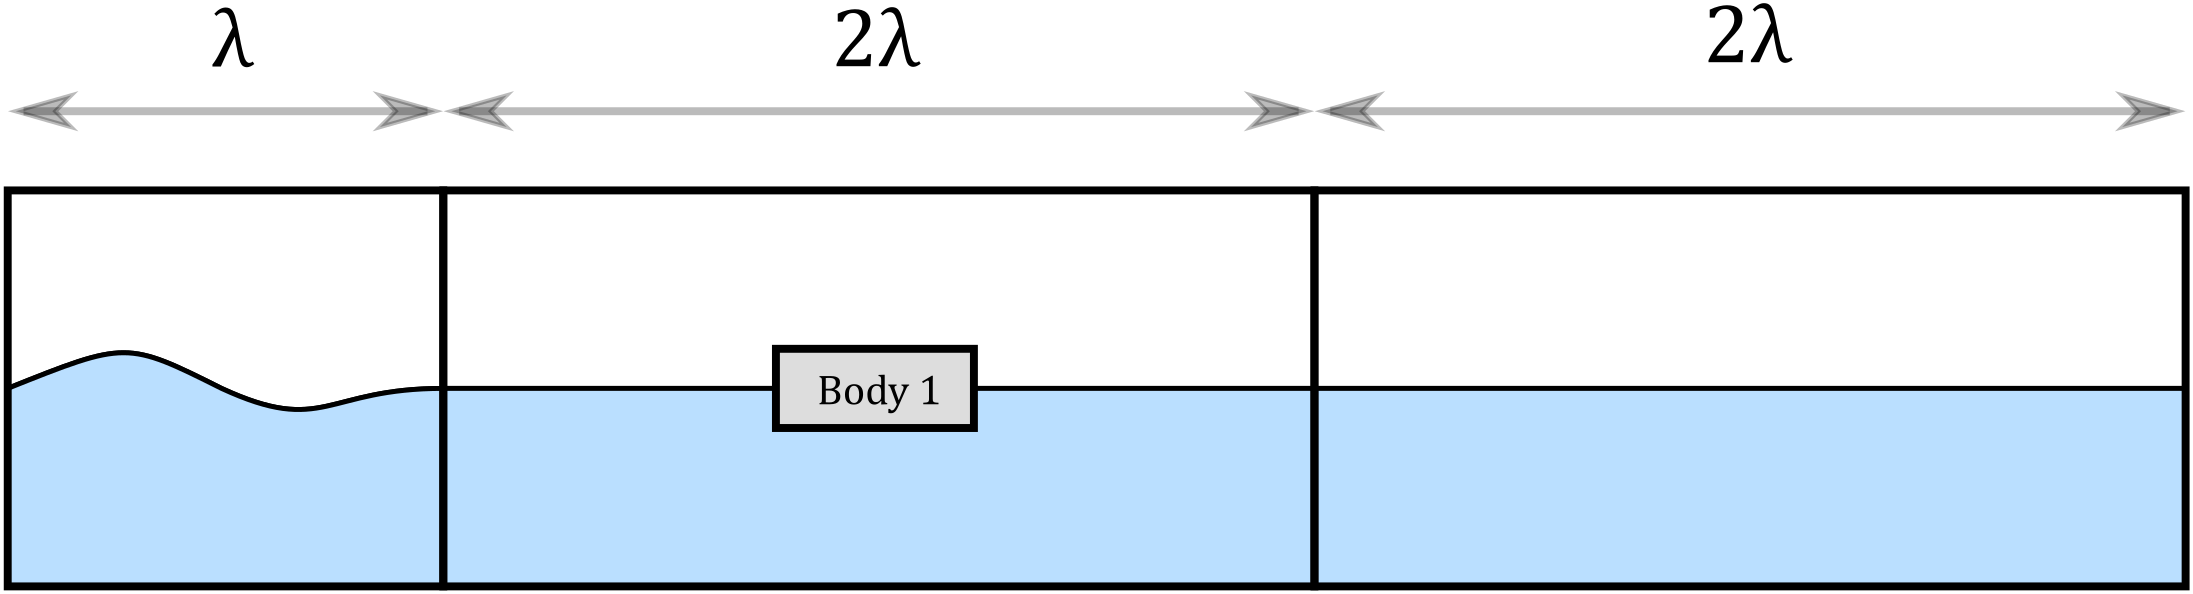
\includegraphics[width=15cm]{floating_body.png}
  \setcaptionwidth{13cm}
  \caption{Geometry of the floating\_body.py case}
  \label{floating_body}
\end{figure}
\newline
This case will be modified in the following steps:
\begin{itemize}
\item translate the first geometry -0.25m in the x-direction
\item add another geometry that lies 0.5m (x-direction) away from the first object
\item connect both bodies with a TSDA
\end{itemize}
\begin{figure}[h]
  \centering
  \includegraphics[width=15cm]{TSDA_title.png}
  \setcaptionwidth{15cm}
  \caption{Geometry of the modified case}
  \label{TSDA_connected_bodies}
\end{figure}
\newpage
\section{Configuration}
This section describes how to add the gmsh pathway to your environment variables. \newline \newline
When you download the gmsh folder, you will see an gmsh.exe file located in the directory that you can double-click on to open gmsh. If you are trying to run gmsh from a windows terminal, you may also want to configure your environment so that the path of gmsh is known. (If you are unfamiliar with path and environment variables, see the documentation below). \newline \newline
https://superuser.com/questions/284342/what-are-path-and-other-environment-variables-and-how-can-i-set-or-use-them \newline \newline
Without specifying the path of gmsh, you would need to specify the path everytime you wanted to run gmsh from your terminal. For example, if my gmsh.exe file was located at: \begin{verbatim}
C:\Users\BarrDaniel\Downloads\gmsh-4.7.0-Windows64\gmsh-4.7.0-Windows64 \end{verbatim}  
, then I would need to type or copy/paste that entire pathway every single time that I wanted to run gmsh from my terminal. If you want to simply type ``gmsh'' in your terminal, you will need to edit your environment variables to include the pathway to this executable file. You can edit your pathway by searching for ``edit environment'' in the windows search box. \newline
\begin{figure}[h]
  \centering
  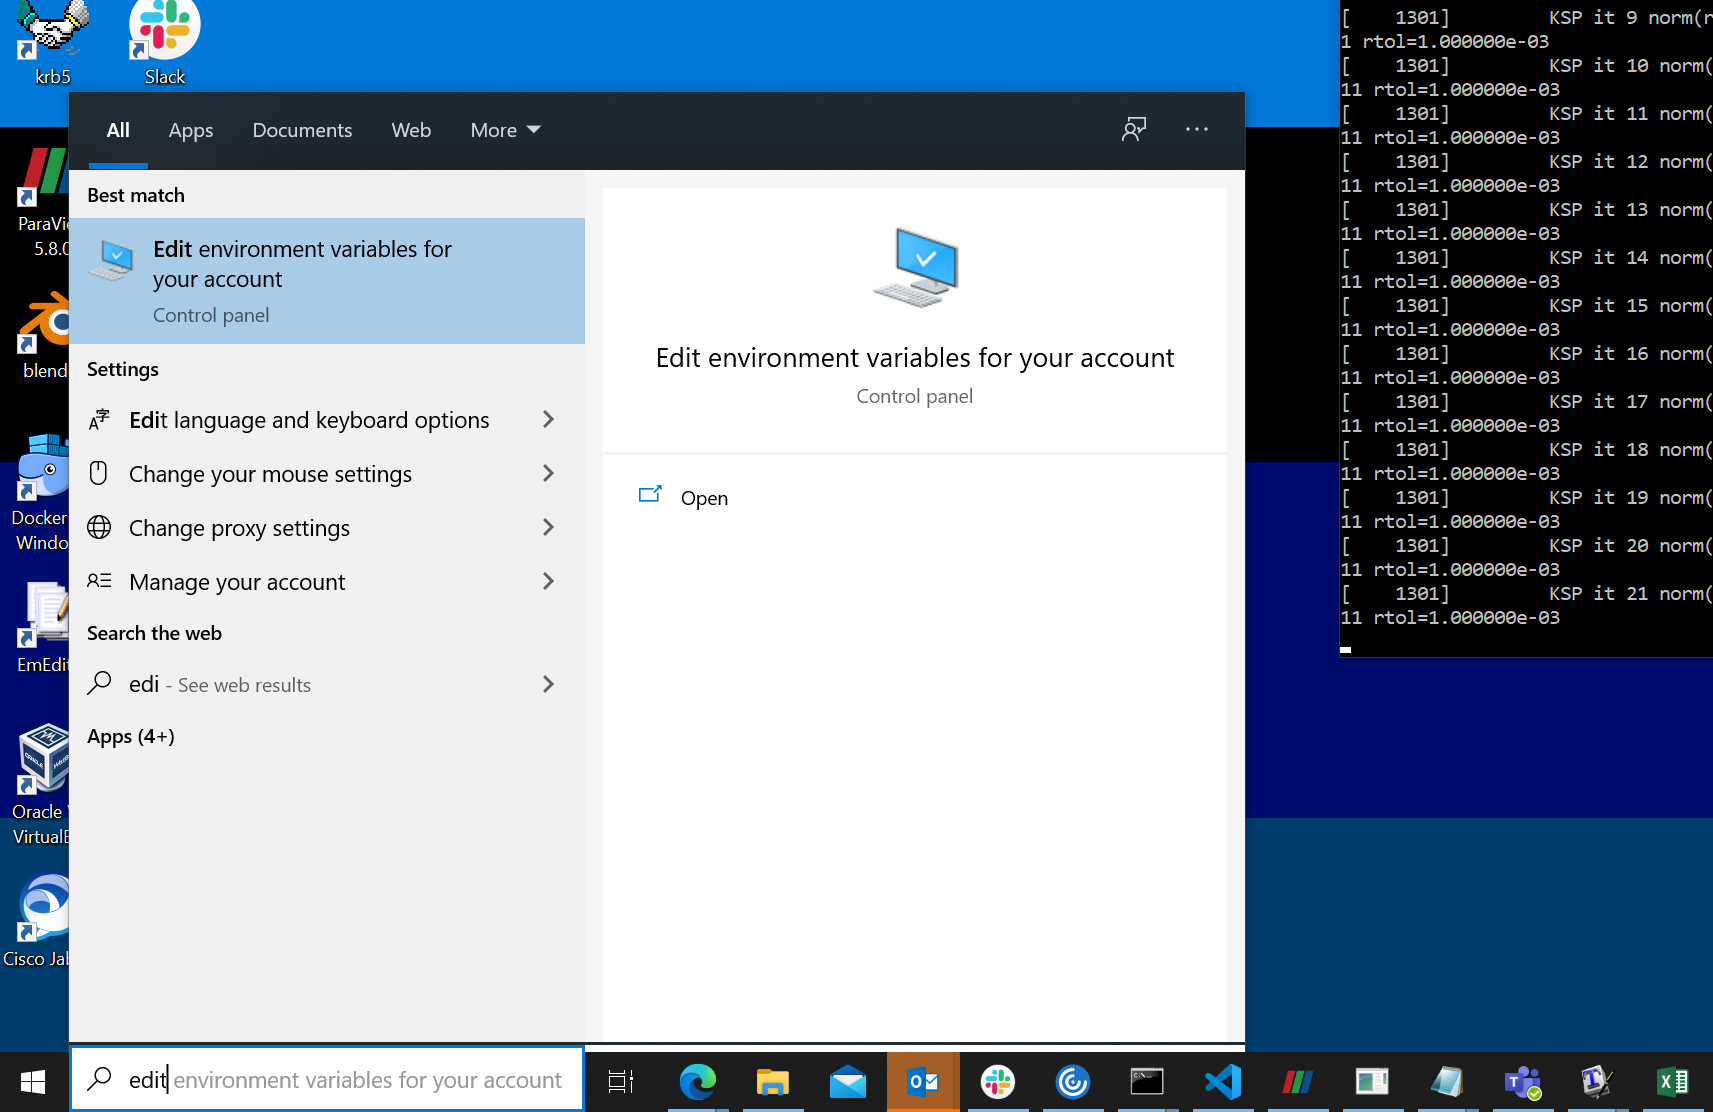
\includegraphics[width=15cm]{EditEnviron.png}
  \setcaptionwidth{15cm}
  \caption{Edit Environment Variables: Step 1}
  \label{TSDA_connected_bodies}
\end{figure}

\noindent (See images on next page for visualization of next steps) Click on ``Path'', then ``Edit'' to edit and add a new path. After this, you can add a new path by clicking on New, then pasting the pathway to your gmsh.exe file. Click ``OK'' then ``OK'' again in the next dialog box, and now your gmsh.exe should be added to your environment variables.

\newpage

\begin{figure}[h]
  \centering
  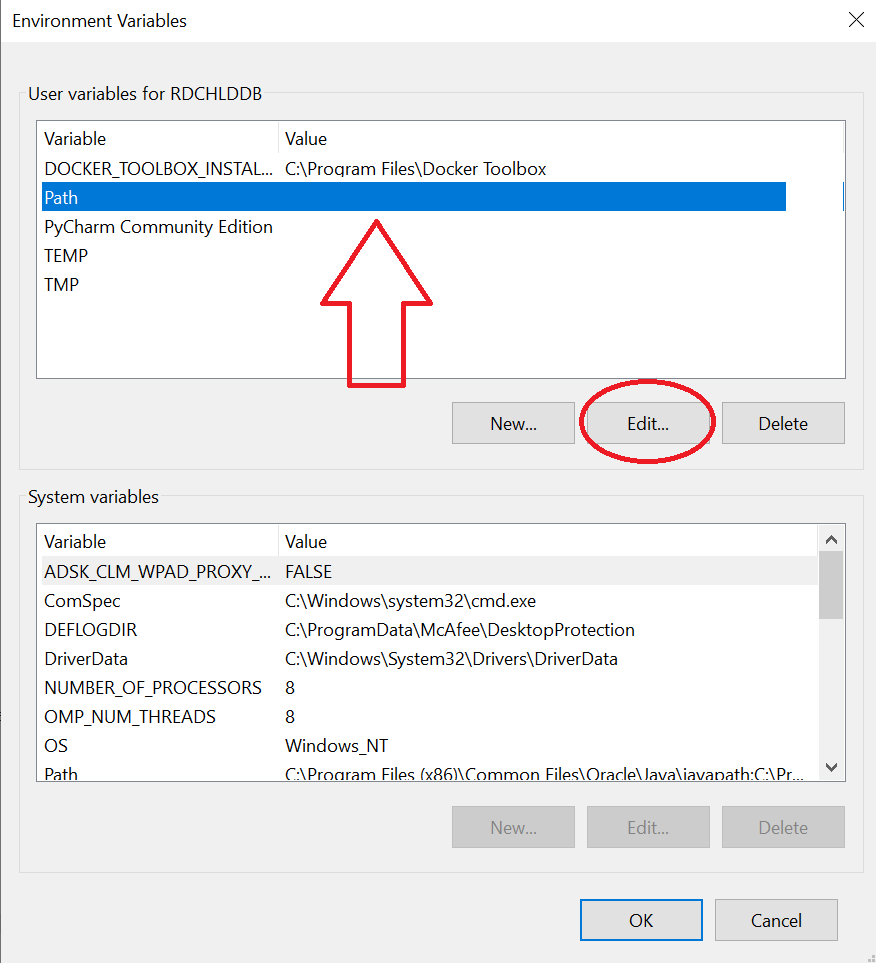
\includegraphics[width=8cm]{EditEnviron2.png}
  \setcaptionwidth{10cm}
  \caption{Edit Environment Variables: Step 2}
  \label{TSDA_connected_bodies}
\end{figure}
\begin{figure}[h]
  \centering
  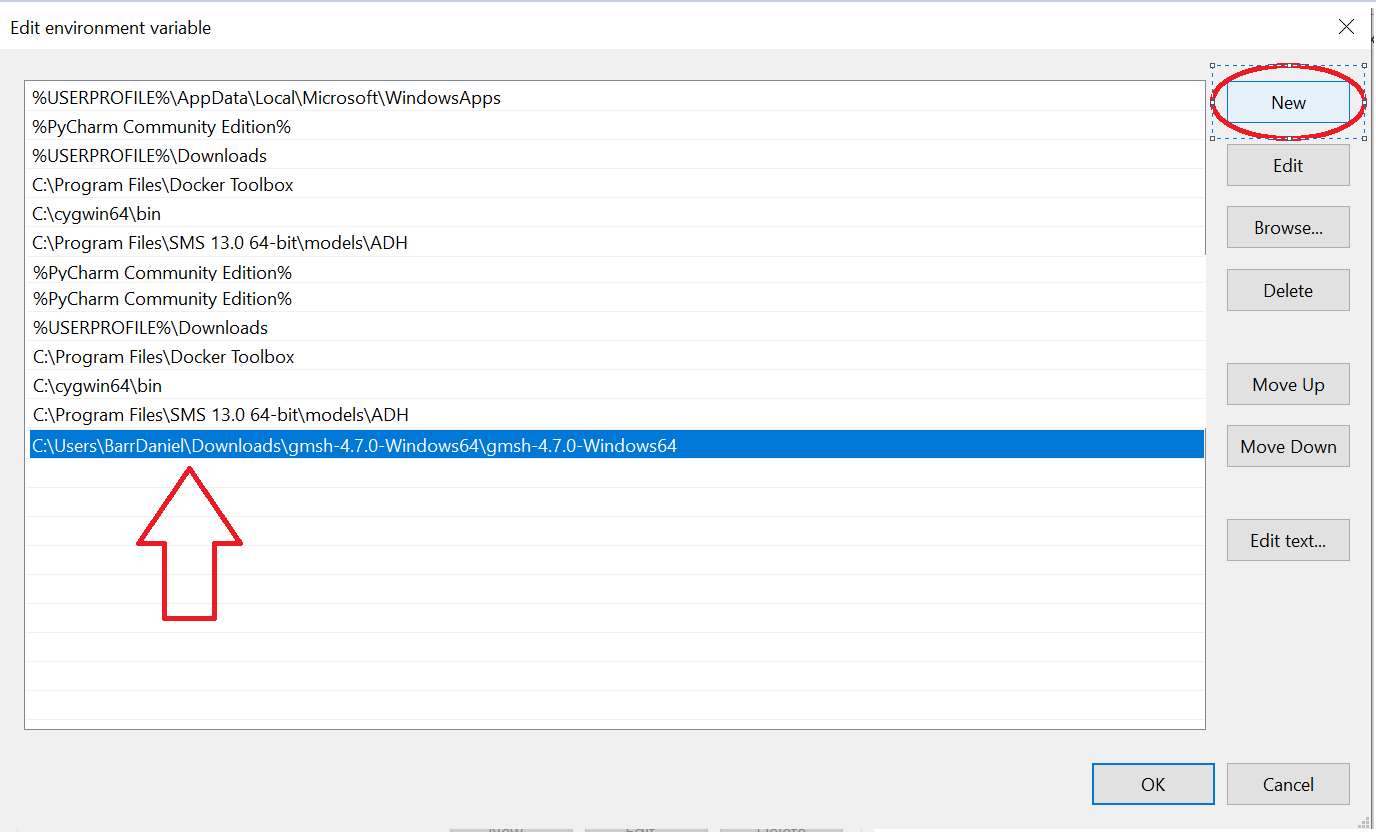
\includegraphics[width=10cm]{EditEnviron3.png}
  \setcaptionwidth{10cm}
  \caption{Edit Environment Variables: Step 3}
  \label{TSDA_connected_bodies}
\end{figure}

\newpage
\section{Creating the 2nd Floating Body}
\subsection{Creating a Second Hole in the Geometry}
If you did not download the proteus\_tutorial folder from this tutorial location, you can git clone it through the command
{
\color{myred}
\begin{verbatim}
git clone https://github.com/erdc/proteus_tutorial        	
\end{verbatim} 
}
\noindent Enter into the appropriate directory and make a copy of the floating\_body case
{
\color{myred}
\begin{verbatim}
cd proteus_tutorial/2D
cp floating_body.py TSDA_connected_bodies.py        	
\end{verbatim} 
}
\noindent After doing this, you should have a copy of the floating\_body.py file that you can edit with whatever text editor that you prefer. Open the TSDA\_connected\_bodies.py file and find the section where the caisson geometry hole is created in the domain. See Listing 1.1 below:
\lstset{language=Python}
\lstset{basicstyle=\fontfamily{pcr}\selectfont\footnotesize\color{red}}
\lstset{backgroundcolor=\color{mygray}}
\lstset{commentstyle=\color{mygreen}}
\lstset{keywordstyle=\color{mycer}}
\lstset{rulecolor=\color{Cerulean}}
\lstset{frame=lines}
\lstset{caption={Script for importing and translating caisson geometry}}
\lstset{label={lst:code_direct}}
\lstset{basicstyle=\footnotesize}
\begin{lstlisting}
caisson = st.Rectangle(domain, dim=(0.5, 0.2), coords=(0., 0.))
# set barycenter in middle of caisson
caisson.setBarycenter([0., 0.])
# caisson is considered a hole in the mesh
caisson.setHoles([[0., 0.]])
# 2 following lines only for py2gmsh
caisson.holes_ind = np.array([0])
tank.setChildShape(caisson, 0)
# translate caisson to middle of the tank
caisson.translate(np.array([1*wavelength, water_level]))
\end{lstlisting}
% 
The first goal here is to shift the first caisson to the left by -0.5. Afterwards, create a second caison and translate it to a distance of 0.5 meters away from the first caisson. Try it for yourself, then double check your code against Listing 1.2.
%
\lstset{language=Python}
\lstset{frame=lines}
\lstset{caption={Script for creating second caisson geometry}}
\lstset{label={lst:code_direct}}
\lstset{basicstyle=\footnotesize}
\begin{lstlisting}
caisson1 = st.Rectangle(domain, dim=(0.5, 0.2), coords=(0., 0.))
# set barycenter in middle of caisson
caisson1.setBarycenter([0., 0.])
# caisson is considered a hole in the mesh
caisson1.setHoles([[0., 0.]])
# 2 following lines only for py2gmsh
caisson1.holes_ind = np.array([0])
tank.setChildShape(caisson1, 0)
# translate caisson to middle of the tank
caisson1.translate(np.array([1*wavelength-0.5, water_level]))

caisson2 = st.Rectangle(domain, dim=(0.5, 0.2), coords=(0., 0.))
# set barycenter in middle of caisson
caisson2.setBarycenter([0., 0.])
# caisson is considered a hole in the mesh
caisson2.setHoles([[0., 0.]])
# 2 following lines only for py2gmsh
caisson2.holes_ind = np.array([0])
tank.setChildShape(caisson2, 0)
# translate caisson to middle of the tank
caisson2.translate(np.array([1*wavelength+0.5, water_level]))
\end{lstlisting}
\newpage
\noindent Additionally, don't forget to update the boundary conditions. Since you possibly changed the name of the first caisson, and you definitely added a new caisson, you will want to make sure this section is updated, as shown in the example below:
\lstset{caption={Script for updated boundary conditions}}
\begin{lstlisting}
for tag, bc in caisson1.BC.items():
    bc.setNoSlip()
for tag, bc in caisson2.BC.items():
    bc.setNoSlip()
\end{lstlisting}
% 	
 After doing these steps, a second hole should have been added to the domain.
\begin{figure}[h]
  \centering
  
\includegraphics[width=15cm]{2_floating_bodies.png}
  \setcaptionwidth{13cm}
  \caption{Updated fluid domain after adding second caisson}
  \label{floating_body}
\end{figure}
\newpage
\subsection{Adding the Second Chrono Body}
Now that the second rectangular hole has been created in the domain, the second chrono body needs to be created, and the first chrono body needs to be updated (assuming you changed the name of the first caisson). All we have done up to this point is create a new hole; however, we have not created the new chrono body and attached the caisson shape to this. You may already know how to do this, so go ahead and try it for yourself. An example of this being done is shown below.
\lstset{language=Python}
\lstset{frame=lines}
\lstset{caption={Script for creating second ChBody and attaching caisson2 (as well as updated caisson1)}}
\lstset{label={lst:code_direct}}
\lstset{basicstyle=\footnotesize}
\begin{lstlisting}
# create floating body
body = fsi.ProtChBody(system=system)
# give it a name
body.setName(b'my_body1')
# attach shape: this automatically adds a body at the barycenter of the caisson shape
body.attachShape(caisson1)
# set 2D width (for force calculation)
body.setWidth2D(0.29)
# access chrono object
chbody = body.getChronoObject()
# impose constraints
chbody.SetBodyFixed(fixed)
free_x = np.array([0., 1., 0.]) # translational
free_r = np.array([0., 0., 1.]) # rotational
body.setConstraints(free_x=free_x, free_r=free_r)
# access pychrono ChBody
# set mass
# can also be set with:
# body.ChBody.SetMass(14.5)
body.setMass(14.5)
# set inertia
# can also be set with:
# body.ChBody.setInertiaXX(pychrono.ChVectorD(1., 1., 0.35))
body.setInertiaXX(np.array([1., 1., 0.35]))
# record values
body.setRecordValues(all_values=True)

# create floating body
body = fsi.ProtChBody(system=system)
# give it a name
body.setName(b'my_body2')
# attach shape: this automatically adds a body at the barycenter of the caisson shape
body.attachShape(caisson2)
# set 2D width (for force calculation)
body.setWidth2D(0.29)
# access chrono object
chbody = body.getChronoObject()
# impose constraints
chbody.SetBodyFixed(fixed)
free_x = np.array([0., 1., 0.]) # translational
free_r = np.array([0., 0., 1.]) # rotational
body.setConstraints(free_x=free_x, free_r=free_r)
# access pychrono ChBody
# set mass
# can also be set with:
# body.ChBody.SetMass(14.5)
body.setMass(14.5)
# set inertia
# can also be set with:
# body.ChBody.setInertiaXX(pychrono.ChVectorD(1., 1., 0.35))
body.setInertiaXX(np.array([1., 1., 0.35]))
# record values
body.setRecordValues(all_values=True)
\end{lstlisting}
\newpage 
\noindent Try running the file, which is now setup to generate waves crashing into 2 floating bodies until t=10s.
{\color{myred}
\begin{verbatim}
parun --TwoPhaseFlow -v -l 5 TSDA_connected_bodies.py        	
\end{verbatim} 
}
\noindent After the simulation completes, you can view the results in paraview by opening the TSDA\_connected\_bodies.xmf file. Below is an example snapshot of the fluid domain with a VOF contour displayed. \newline
\begin{figure}[h]
  \centering
  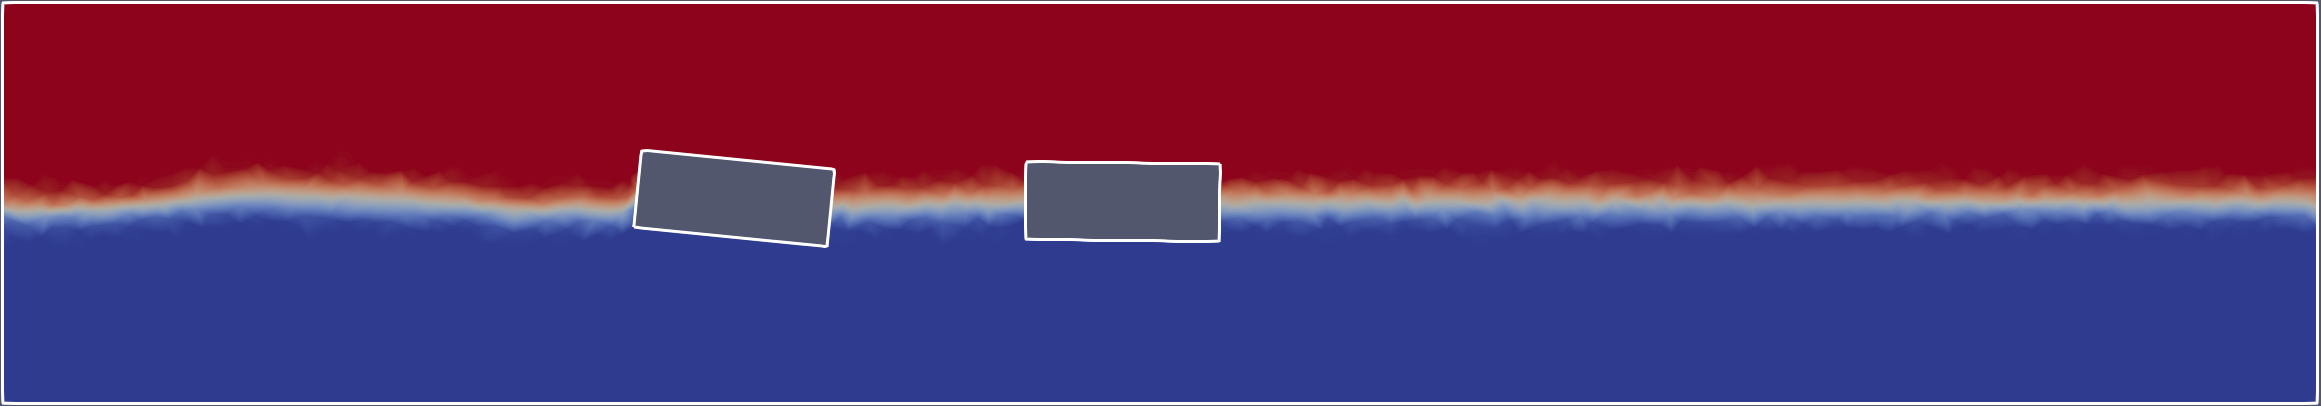
\includegraphics[width=15cm]{2_floating_bodies_2.png}
  \setcaptionwidth{13cm}
  \caption{Two unconnected floating bodies at t=9.26s}
  \label{floating_body}
\end{figure}

\noindent Copy these files into a new directory so that we can use it to compare results at a later time.
{
\color{myred}
\begin{verbatim}
mkdir unconnected_bodies
cp TSDA_connected_bodies* unconnected_bodies/.
cp rectangle* unconnected_bodies/.
\end{verbatim} 
}
\newpage
\section{Setting up the TSDA in proteus}
\lstset{caption={Script for creating the TSDA in proteus}}
\begin{lstlisting}
# create the ChLinkTSDA
TSDA = pychrono.ChLinkTSDA() 
# store the location of the connection on the first body
body1_point = pychrono.ChVectorD(wavelength-0.25,water_level+0.1,0.0)  
# store the location of the connection on the second body
body2_point = pychrono.ChVectorD(wavelength+0.25,water_level+0.1,0.0)   

# initialize the system
TSDA.Initialize(system.subcomponents[0].ChBody,system.subcomponents[1].ChBody,
                      False,
                      body1_point, 
                      body2_point, 
                      auto_rest_length=True)

# Set a constant coefficient for the spring
TSDA.SetSpringCoefficient(400.)

#Add the TSDA to the system
system.ChSystem.Add(TSDA)
\end{lstlisting}
\newpage
\section{Logging the TSDA Information}

\newpage

\chapter{Basic GUI Functionality}
\section{Navigating and Meshing}

\newpage
\section{Finding Low Quality Elements in the Mesh}

\chapter{Other Useful Links}
\section{Manual}
\section{tutorials}

\begin{figure}[h]
  \centering
  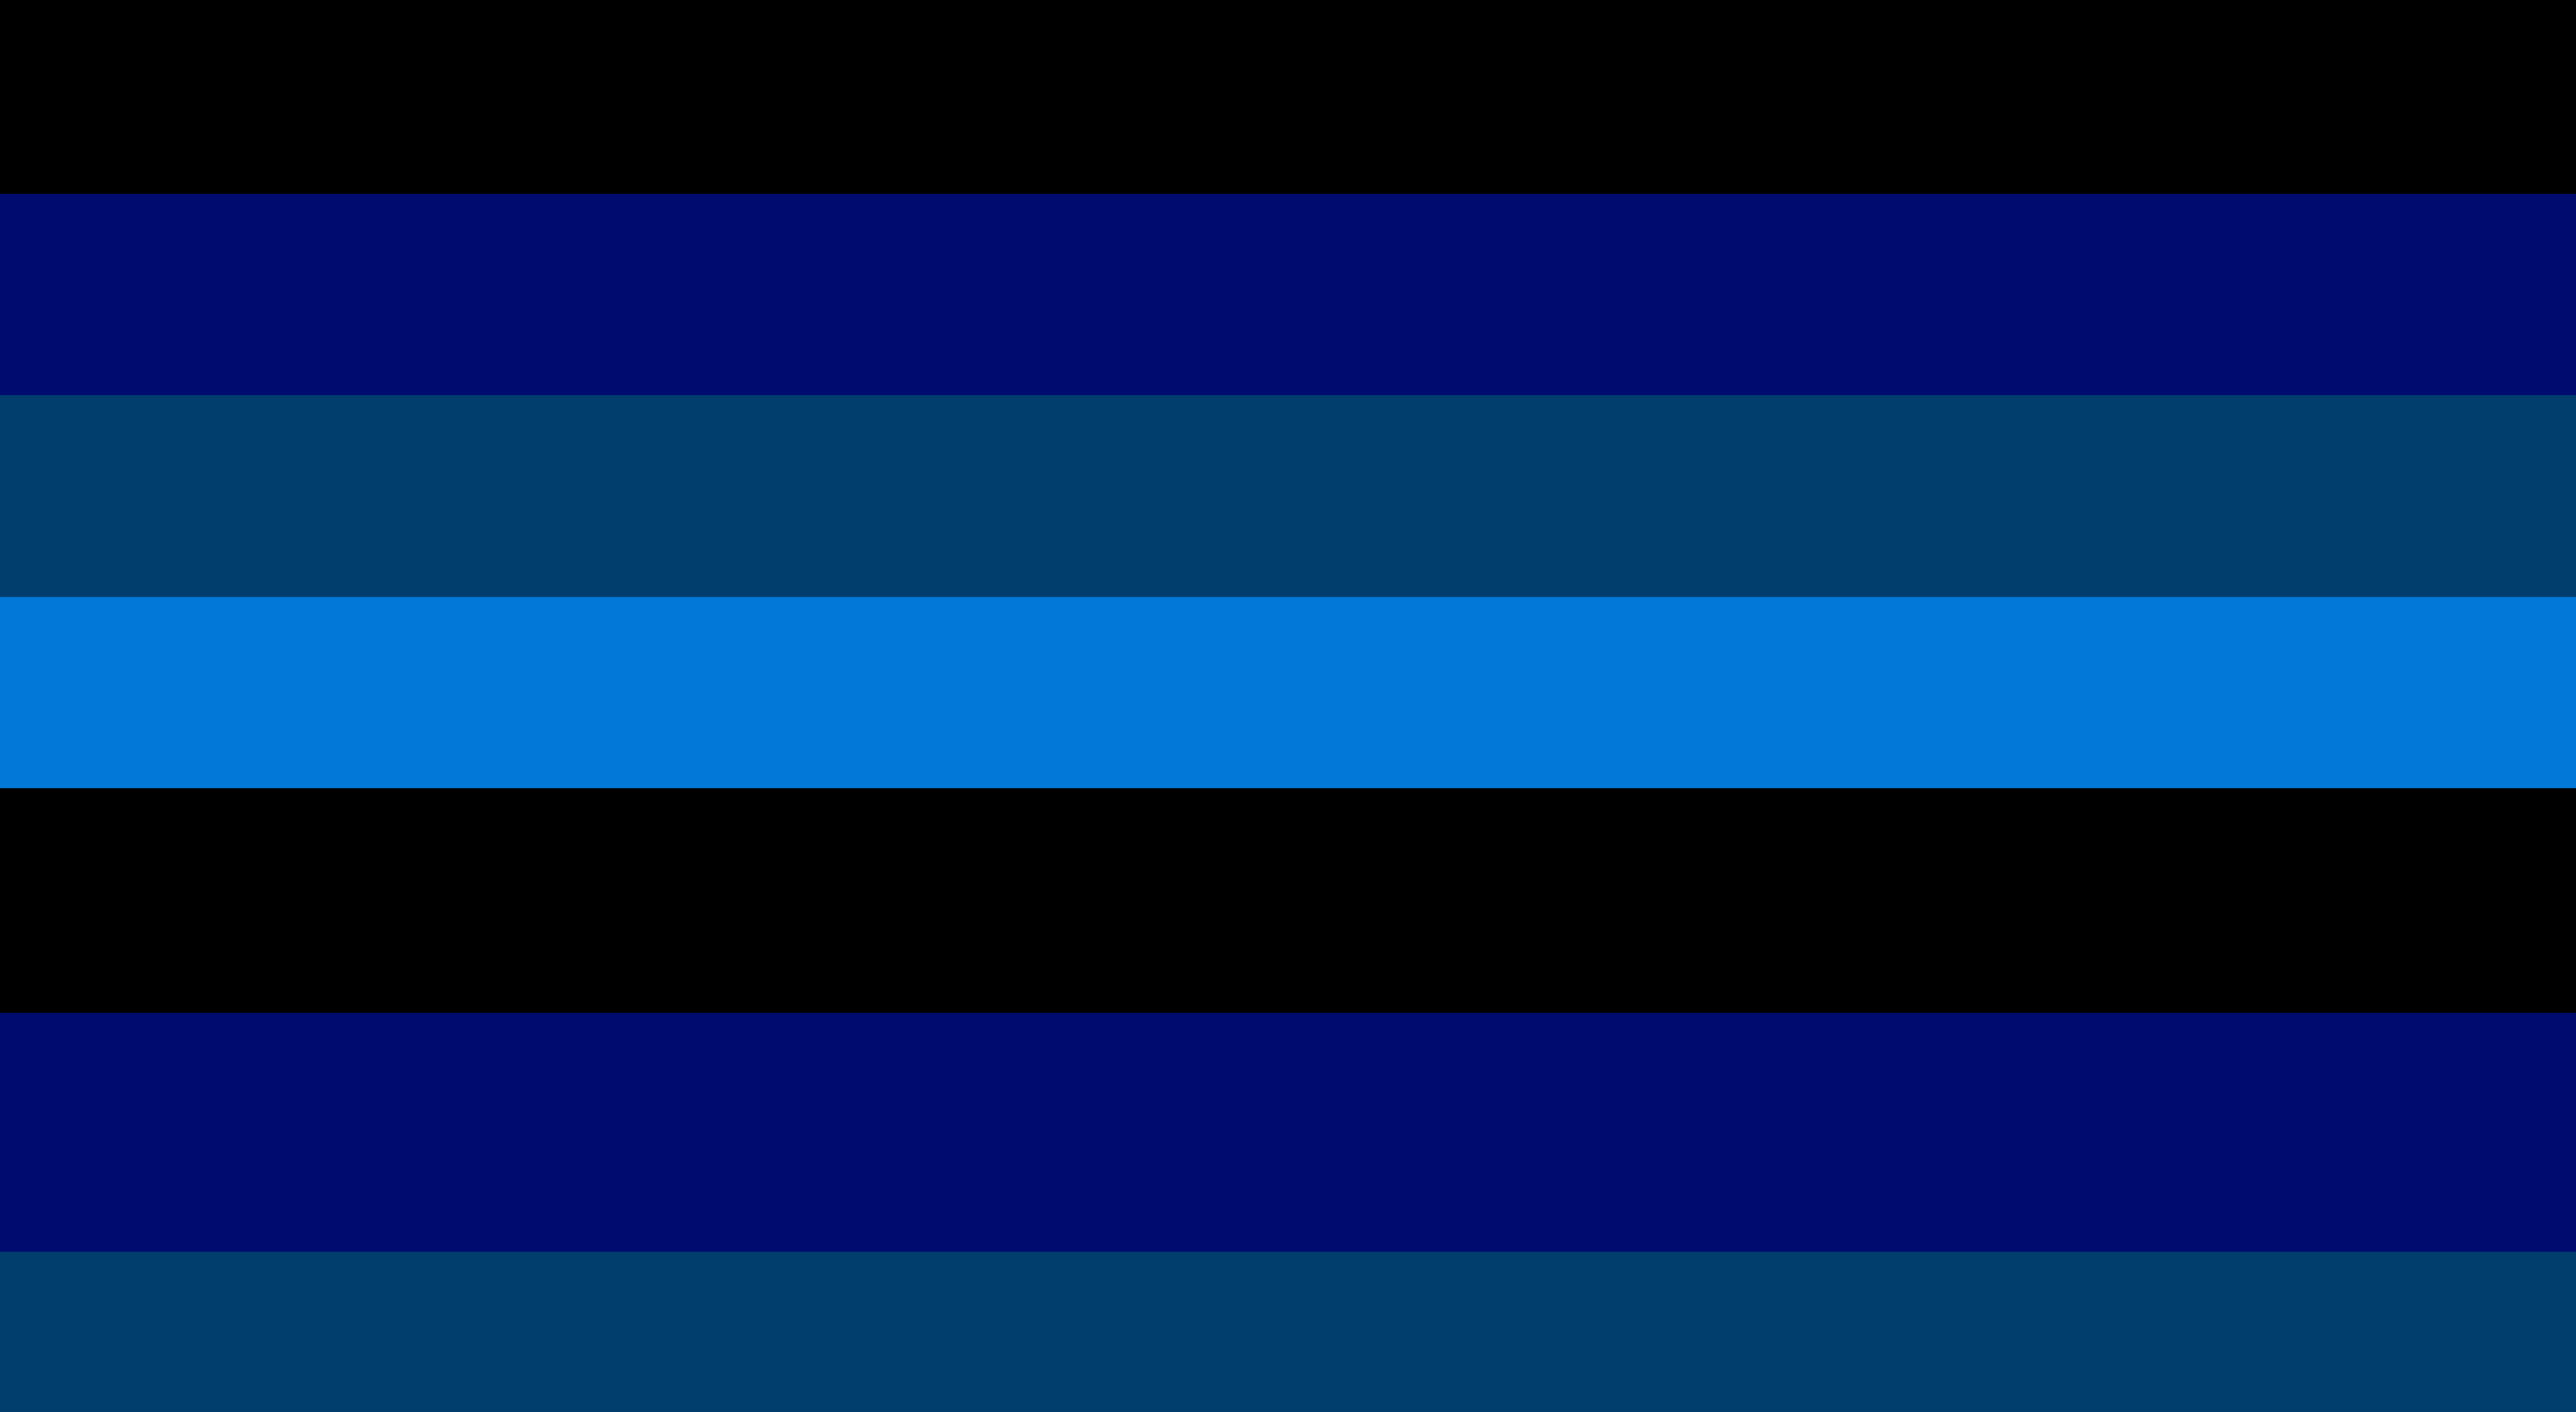
\includegraphics[width=4cm]{geo1.png}
  \setcaptionwidth{14cm}
  \caption{Geometry of the dieseFoam tutorial case.}
  \label{geo1}
\end{figure}
\newpage


\end{document}
